\chapter{背景知识与相关技术}
\label{chap:background}

本章介绍了物联网设备固件仿真研究涉及的基础知识与技术工具。首先阐述物联网设备的硬件架构与驱动软件模型（第~\ref{sec:hw}~和~\ref{sec:os}~节），明确固件与硬件交互的底层机制；然后介绍静态分析技术（第~\ref{sec:program-analysis}~节）和固件仿真与模糊测试技术（第~\ref{sec:fuzz}~节），为驱动函数的识别与动态验证提供方法支撑；最后介绍大语言模型代码分析智能体框架（第~\ref{sec:llm}~节），为解决传统方法自动化程度不足的问题提供技术途径。上述内容为后续章节的系统设计与实现奠定基础。

\section{物联网设备硬件基础}
\label{sec:hw}

物联网设备通常采用嵌入式微控制器（Microcontroller Unit, MCU）作为核心处理器。常见的 MCU 架构包括 ARM Cortex-M 系列、RISC-V 等。这些处理器具有低功耗、低成本、实时性强等特点，广泛应用于物联网领域。本节重点介绍 ARM Cortex-M 架构特性，以及物联网固件外设交互机制的基础内容，涵盖 MMIO、中断与 DMA 三类关键机制。

\subsection{ARM Cortex-M 架构特性}
\label{sec:cortex_m}
ARM Cortex-M 是 ARM 架构处理器核心中低端系列的统称，专为低成本、高能效的微控制器设计，广泛应用于物联网设备。该系列采用 Thumb-2 指令集，在提供 32 位性能的同时保持 16 位代码密度。Cortex-M 架构提供了多项增强实时性和可靠性的特性，包括嵌套向量中断控制器（NVIC）用于中断管理、系统定时器用于提供可编程的周期性中断并支持操作系统的任务调度、以及主栈与进程栈的栈模式切换机制以实现多任务并发和内存保护。
\subsection{外设交互机制基础}
\label{sec:mmio}

本小节从寄存器访问、事件响应和数据搬运三个维度介绍外设交互机制，分别对应 MMIO、中断与 DMA。内存映射 I/O（Memory-Mapped I/O, MMIO）是嵌入式系统中外设与处理器通信的主要方式。MMIO 将外设寄存器映射到处理器的统一内存地址空间中，处理器通过普通的内存读写指令（如 \texttt{LDR}/\texttt{STR}）访问特定内存地址，即可完成对外设的控制和数据传输。这种设计简化了编程模型，使得外设访问与内存访问具有相同的语法形式。

ARM Cortex-M 架构采用统一的 32 位地址空间，按功能划分为代码区（Flash）、SRAM 区、外设区和系统区，如图~\ref{fig:memory-map}所示。外设区是 MMIO 的核心区域，所有片上外设的寄存器都被映射到此区域，不同厂商的外设被分配到不同的地址段。系统区位于地址空间高端，包含 NVIC、SysTick、MPU 等系统级组件的控制寄存器。理解 MMIO 地址空间布局对于固件仿真至关重要，仿真器需要针对外设区和系统区实现专门的访问处理逻辑。

\begin{figure}[htbp]
\centering
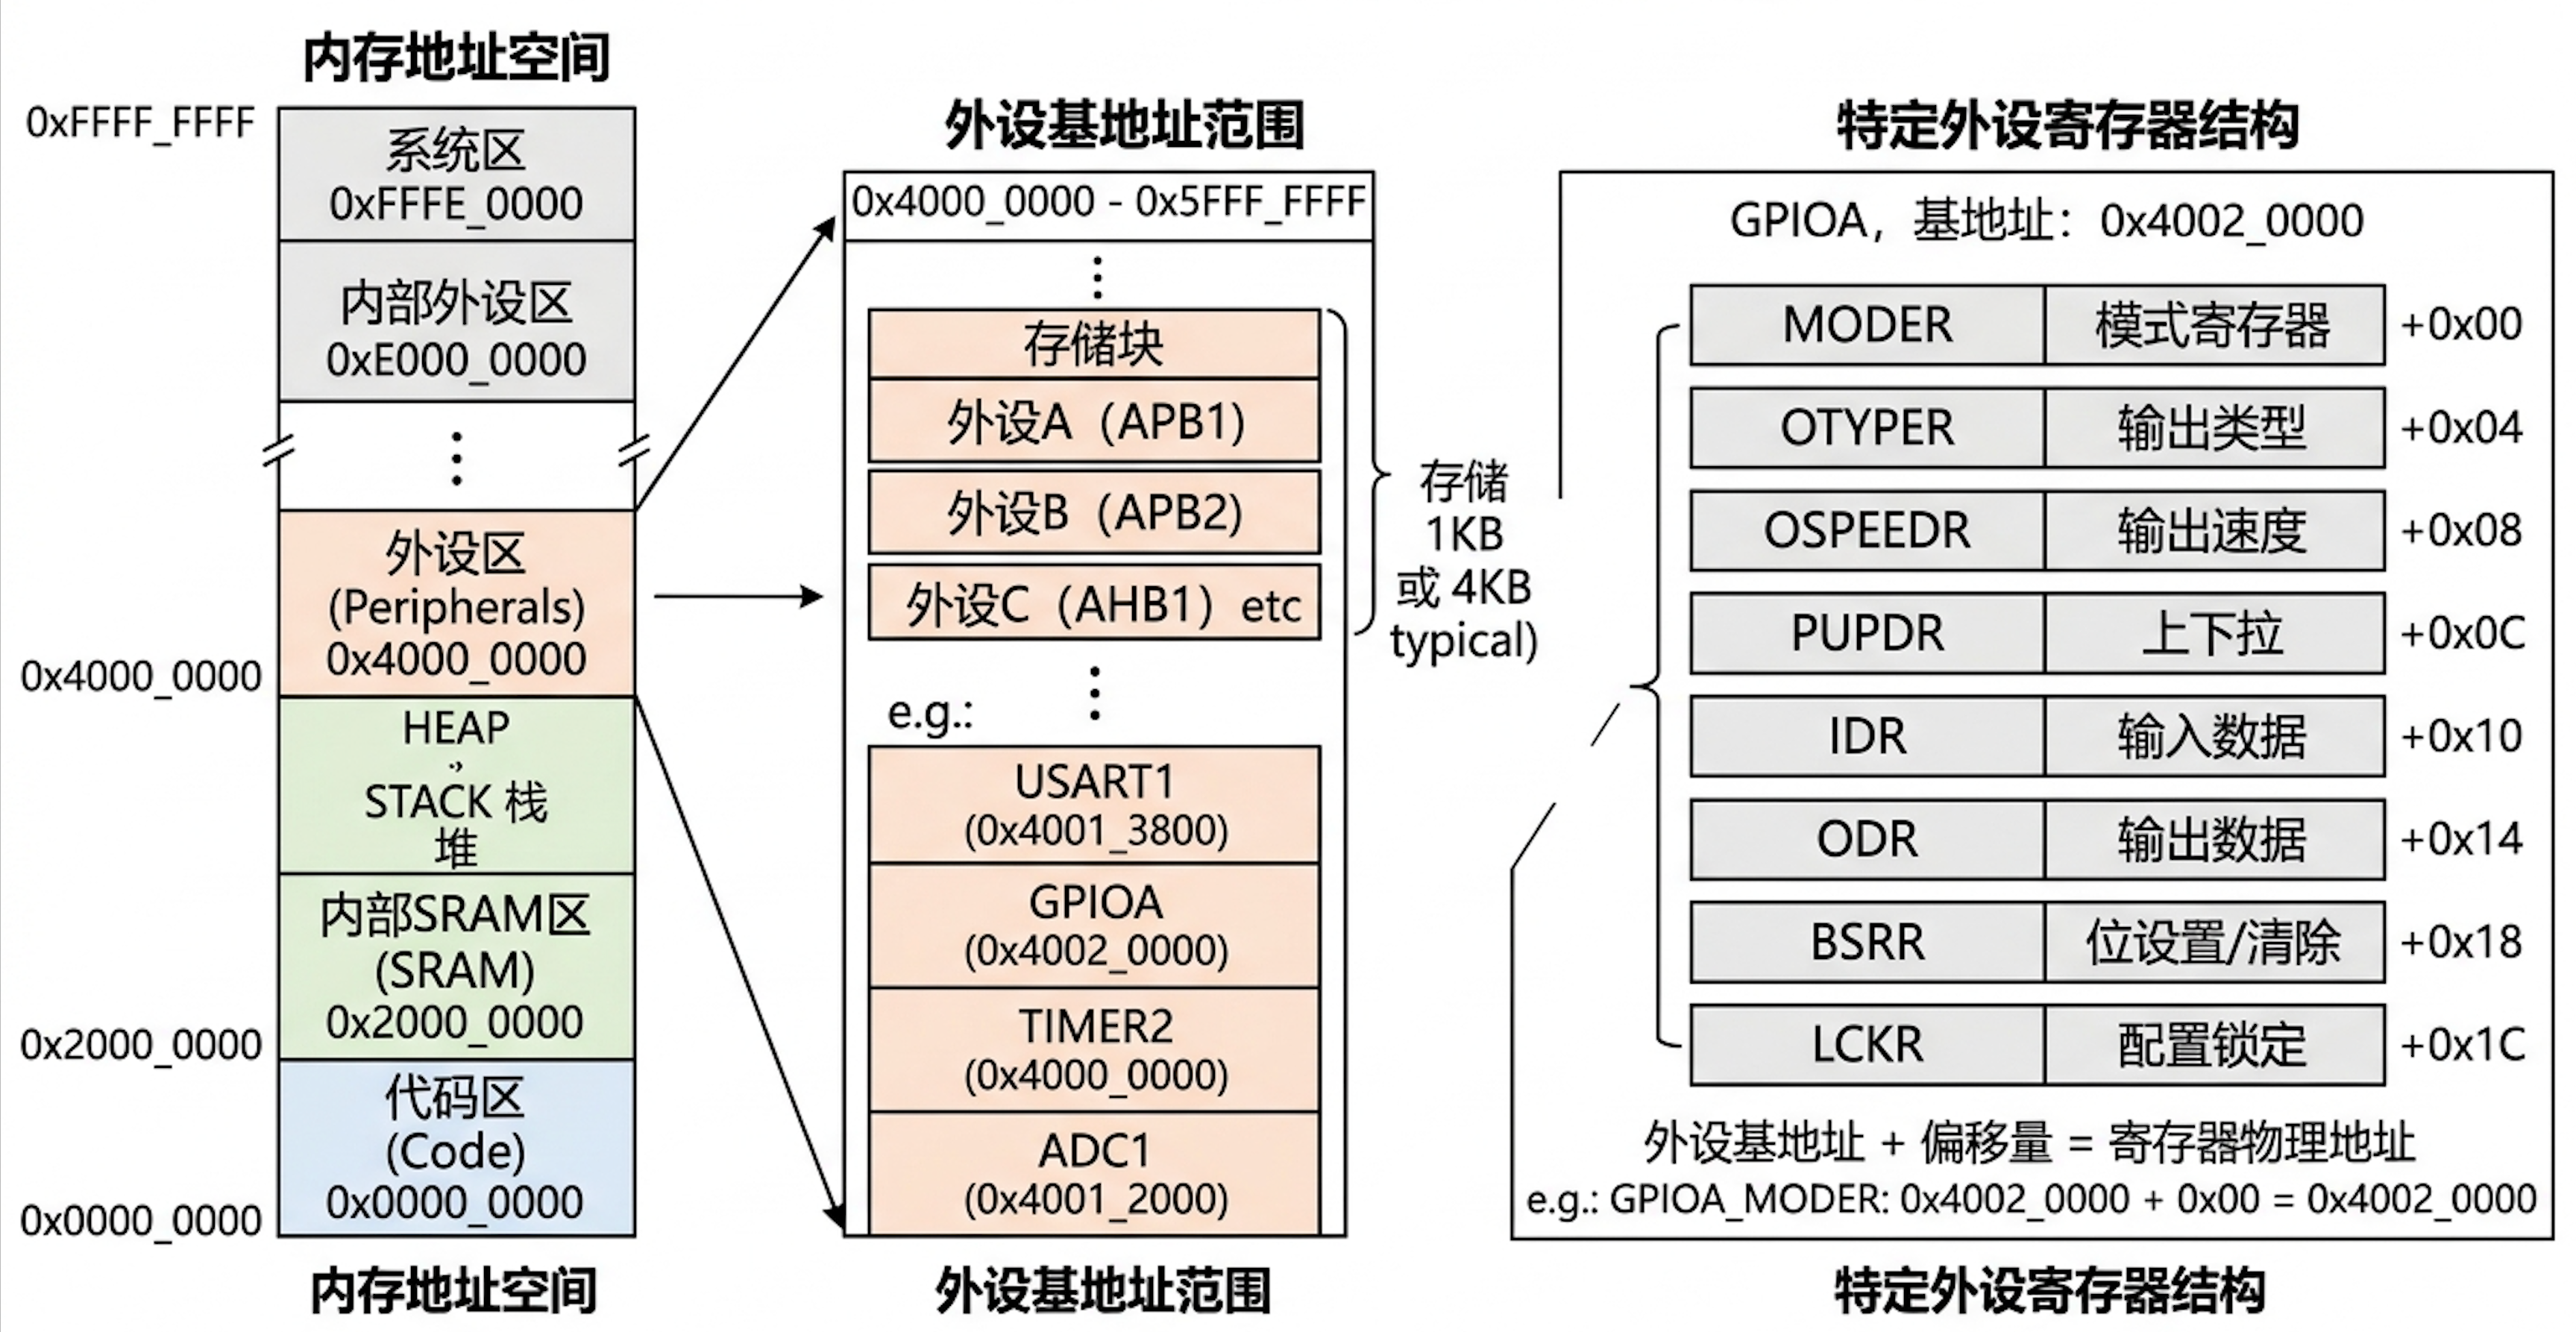
\includegraphics[width=0.85\textwidth]{figures/Arm架构图.png}
\caption{ARM Cortex-M 内存地址空间布局}
\label{fig:memory-map}
\end{figure}

外设寄存器按照功能可分为控制寄存器、状态寄存器和数据寄存器三类。控制寄存器用于配置外设的工作模式和参数，如 USART 的 CR1 可设置波特率、数据位长度等。状态寄存器反映外设的当前工作状态，如 USART 的 SR 包含发送缓冲区空（TXE）、接收缓冲区非空（RXNE）等标志位，其值由硬件自动更新。数据寄存器用于数据传输，如 USART 的 DR 用于发送和接收数据，访问数据寄存器通常会触发外设执行相应操作。

除 MMIO 外，中断（Interrupt）和直接内存访问（Direct Memory Access, DMA）也是嵌入式固件常见的外设操作方式。中断机制通过 NVIC 将外设事件（如串口接收完成、定时器溢出）异步通知给处理器，处理器在中断服务函数中完成状态更新或任务唤醒。DMA 机制允许外设在不经过 CPU 逐字搬运的情况下，直接与内存进行批量数据传输，常用于串口、SPI、ADC 等场景，以降低 CPU 开销并提升吞吐。

在固件仿真与驱动替换场景下，这三种机制往往共同出现：MMIO 负责寄存器读写与状态轮询，中断负责事件驱动控制流切换，DMA 负责高频数据搬运路径。若仅建模 MMIO 而忽略中断和 DMA，可能导致任务调度时序不一致、数据路径不完整或覆盖率评估偏差。因此，后续静态分析与动态验证需要同时关注寄存器访问模式、中断处理路径以及 DMA 相关配置与回调逻辑。

\section{物联网操作系统与驱动}
\label{sec:os}

\subsection{实时操作系统概述}
\label{sec:rtos}

实时操作系统（Real-Time Operating System, RTOS）是物联网设备中广泛采用的管理任务调度和资源分配的软件系统。RTOS 能够及时响应外部事件或数据，并在规定的时间内完成任务，其工作原理是通过一个实时任务调度器来管理系统资源，按照优先级或者时间片来分配 CPU 时间给不同的任务，保证重要或者紧急的任务优先执行。

物联网领域常见的 RTOS 包括 FreeRTOS\cite{freertos}、Zephyr\cite{zephyr}、RT-Thread\cite{rtthread} 等。FreeRTOS 是 Amazon 开源的实时操作系统，专为微控制器和小型微处理器设计，内核精简，最小可运行在不到 10KB 的 RAM 上，是物联网领域使用最广泛的 RTOS 之一。Zephyr 是 Linux 基金会管理的开源实时操作系统，支持多种处理器架构，提供更完整的操作系统功能，包括文件系统、网络协议栈、设备驱动模型等，采用模块化设计以平衡功能丰富性和资源占用。RT-Thread 是中国开源社区主导开发的实时操作系统，采用微内核架构，并提供了丰富的组件生态。

\begin{figure}[htbp]
\centering
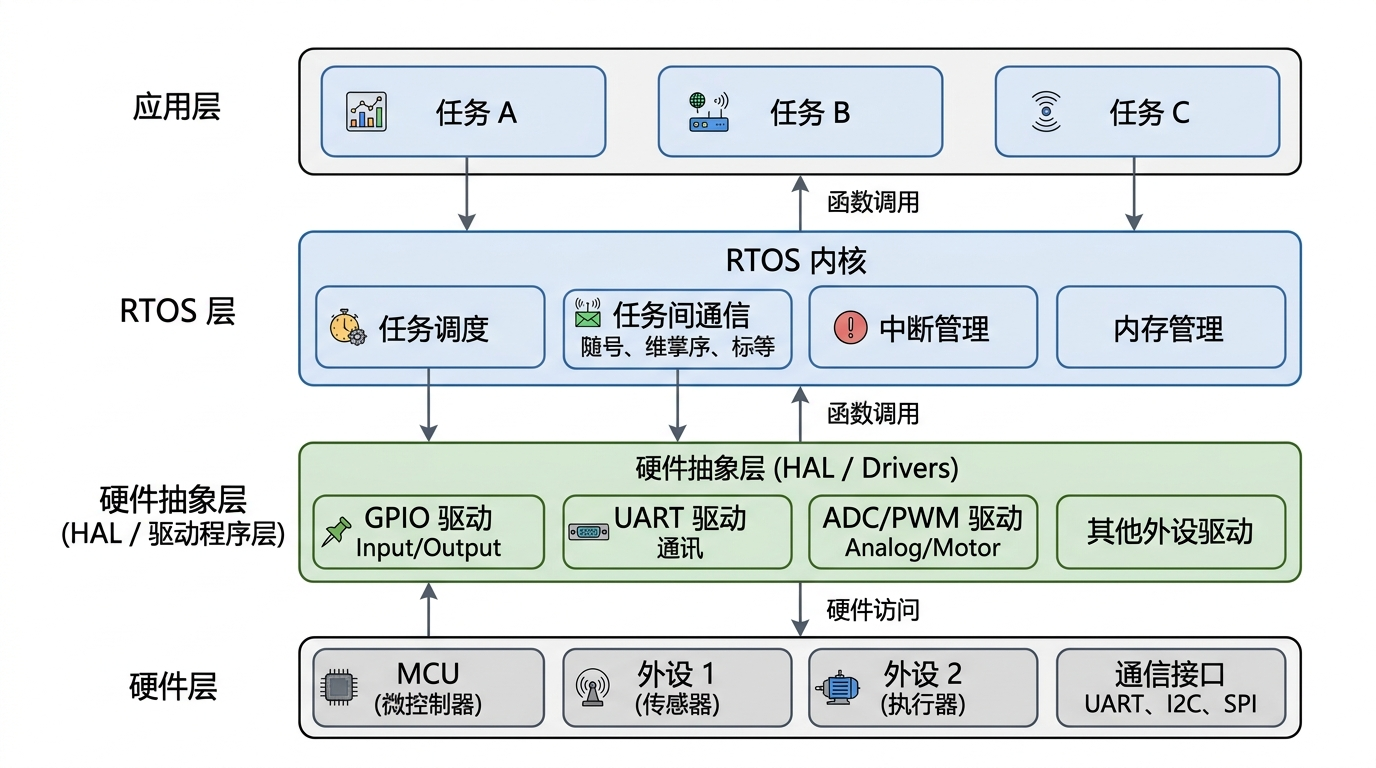
\includegraphics[width=0.85\textwidth]{figures/搭载RTOS的嵌入式固件的系统架构图.png}
\caption{搭载 RTOS 的嵌入式固件系统架构图}
\label{fig:rtos-arch}
\end{figure}

搭载 RTOS 的嵌入式固件通常采用分层架构，如图~\ref{fig:rtos-arch}所示。整个系统自底向上依次为硬件层、硬件抽象层（HAL）、操作系统内核以及应用层。硬件层包含 MCU 及各类外设；HAL 层封装了对底层寄存器的访问细节；RTOS 内核负责任务调度、中断管理和资源分配；应用层则实现具体的业务逻辑。固件运行过程中，应用程序通过 RTOS 提供的系统调用和驱动接口访问硬件资源，而非直接操作寄存器。这种分层结构使得驱动函数替换成为可能：仿真器可以在 HAL 层或驱动框架层拦截函数调用，用宿主机侧实现替代原始的硬件操作，从而在不修改上层应用逻辑的前提下实现固件的仿真执行。

\subsection{硬件抽象层}
\label{sec:hal}

硬件抽象层（Hardware Abstraction Layer, HAL）是嵌入式软件架构中的关键组成部分，它位于硬件驱动层和上层应用之间，为应用程序提供统一的硬件访问接口。HAL 层的核心目标是屏蔽底层硬件的差异性，使得上层应用代码可以在不同的硬件平台之间移植，而无需修改业务逻辑。

HAL 层的接口设计遵循统一的命名和功能规范。以 STM32 HAL 库为例，每个外设类型提供初始化函数（如 \texttt{HAL\_UART\_Init}）、数据传输函数（如 \texttt{HAL\_UART\_Transmit}）、状态查询函数（如 \texttt{HAL\_UART\_GetState}）和中断管理函数（如 \texttt{HAL\_UART\_Receive\_IT}）。由于 HAL 函数封装了底层硬件操作细节，仿真器可通过替换 HAL 层函数来实现硬件行为模拟，无需深入理解寄存器语义，相比寄存器级模拟更加高效且易于实现。

\section{开源程序静态分析技术}
\label{sec:program-analysis}

前两节介绍了物联网设备的硬件架构和驱动软件分层模型，明确了固件中驱动函数与硬件交互的基本方式。要实现驱动函数的自动化分析和替换，首先需要一种能够精确识别代码中 MMIO 访问模式和函数间数据流关系的分析手段。在静态分析引擎的选型上，本文考量了基于 LLVM/Clang 和基于 CodeQL 两种方案：基于 LLVM/Clang 的方案需要将嵌入式固件的构建工具链从 ARM GCC 切换到 Clang，而 CMSIS 头文件、厂商设备描述头文件以及 \texttt{\_\_attribute\_\_}、\texttt{\_\_IO} 等 ARM GCC 扩展语法在 Clang 下的兼容性尚不完整，迁移成本较高；CodeQL 通过在构建过程中拦截编译器调用来捕获源码信息，无需替代原始编译器，可直接在 ARM GCC 工具链上工作，无需修改固件工程的编译配置。基于上述分析，本研究选择 CodeQL 作为静态分析引擎，本节介绍其核心原理。

\subsection{CodeQL 代码分析平台}

CodeQL 是 GitHub 开发的语义级代码分析平台，支持多种编程语言（包括 C/C++、Java、Python、JavaScript 等）的安全漏洞检测和代码质量分析。CodeQL 的核心思想是将源代码转换为可查询的数据库，然后通过声明式查询语言（QL）进行灵活的分析。与传统基于规则的静态分析工具不同，CodeQL 提供了表达力丰富的查询语言，研究人员可以通过编写查询来查找特定的代码模式、追踪数据流、分析控制依赖等复杂问题。

CodeQL 的工作原理分为两个阶段。第一阶段是数据库构建，CodeQL 对源代码进行解析，生成抽象语法树（AST）、控制流图（CFG）、数据流图（DFG）等多层次的结构化表示，并将这些信息存储在数据库中。第二阶段是查询执行，研究人员使用 QL 语言编写查询，在数据库上执行，获取分析结果。CodeQL 的查询语言基于 Datalog，采用谓词逻辑的表达方式，能够自然地表达“所有存在某种模式的代码片段”或“从源点到汇点的数据流路径”等复杂查询。

CodeQL 在程序分析领域应用广泛，包括安全漏洞检测（如 SQL 注入、缓冲区溢出）、代码质量分析（如死代码检测、复杂度分析）、以及依赖关系分析（如函数调用图、数据流追踪）。本研究利用 CodeQL 的数据流追踪能力，建立 MMIO 访问与函数参数之间的关联关系，为驱动函数识别和语义分析提供支撑。

\section{物联网设备固件仿真与模糊测试}
\label{sec:fuzz}

静态分析能够识别驱动函数及其硬件访问模式，但要验证替换后固件的正确性，还需要将固件在仿真环境中动态执行并进行测试。固件仿真是物联网安全研究的重要技术手段。由于物联网设备的硬件多样性和封闭性，直接在真实设备上进行安全测试面临诸多困难。固件仿真技术通过软件模拟硬件环境，使研究人员能够在通用计算平台上运行和分析嵌入式固件，从而降低测试成本并提高效率。模糊测试作为一种高效的漏洞挖掘技术，与固件仿真相结合，能够在仿真环境中自动化地发现固件中的安全漏洞。

\subsection{QEMU 仿真器}

QEMU\cite{qemu} 是目前应用最广泛的开源机器仿真器，支持多种处理器架构和外设仿真，其设计目标是提供高性能、高可移植性的系统仿真能力，使其成为固件仿真研究的重要基础平台。QEMU 支持两种主要的仿真模式：用户模式仿真（User Mode Emulation）允许在一种架构上运行为另一种架构编译的单个程序，适用于分析用户空间程序；系统模式仿真（System Mode Emulation）提供完整的硬件系统仿真，包括处理器、内存、中断控制器、外设等组件，可以运行完整的操作系统或裸机固件，这是固件仿真的主要工作模式。

QEMU 的核心是动态二进制翻译引擎（Tiny Code Generator, TCG），它将目标架构的指令块翻译为中间表示（IR），然后再将 IR 翻译为宿主机指令，这种两级翻译机制使 QEMU 能够支持多种目标架构和宿主架构的组合。为了提高性能，TCG 采用即时编译（JIT）技术，将翻译结果缓存在内存中供后续执行重复使用。

Unicorn\cite{unicorn} 是基于 QEMU 的 TCG 引擎开发的轻量级 CPU 模拟器，专门针对安全研究和逆向工程场景优化。与 QEMU 提供完整系统级仿真的设计不同，Unicorn 去除了 QEMU 的系统级组件和外设仿真，只保留指令集模拟核心，因此具有更好的灵活性和可控性。Unicorn 提供了丰富的钩子（Hook）机制，允许用户在指令执行、内存访问、中断触发等事件上注册自定义回调函数，从而在不修改模拟器源码的情况下实现对执行过程的细粒度监控和干预。此外，Unicorn 以库的形式提供编程接口（支持 Python、C 等多种语言），便于嵌入到其他工具链中。本研究选用 Unicorn 作为固件动态测试的仿真引擎，利用其 ARM Thumb 模式模拟 ARM Cortex-M 系列微控制器，并通过钩子机制实现驱动函数拦截、运行日志采集和仿真数据注入等功能。



\subsection{模糊测试技术}

模糊测试（Fuzzing）是一种自动化软件测试技术，通过向目标程序输入大量随机、半随机或结构化的测试用例，来发现程序中的安全漏洞和缺陷\cite{manesArtScienceEngineering2021}。模糊测试的基本工作流程包括：生成或变异测试用例、将测试用例输入目标程序、监控程序执行状态（如崩溃、断言失败、内存错误等）、记录和分析异常。

American Fuzzy Lop（AFL）\cite{aflplusplus_paper} 是最具影响力的覆盖率引导模糊测试工具之一。AFL 的核心思想是通过代码插桩技术记录程序执行过程中的覆盖率信息，利用这些信息指导测试用例的变异和选择，优先保留能够触发新执行路径的测试用例，从而在有限的测试时间内探索更多的程序状态，提高漏洞发现的概率。AFL 的工作流程包含两个核心环节：覆盖率记录和变异策略。在覆盖率记录环节，AFL 通过编译时插桩或运行时插桩（利用 QEMU 的动态翻译功能）在目标程序中插入覆盖率记录代码，记录程序执行过程中经过的基本块和边。在变异策略环节，AFL 维护一个测试用例队列，不断从队列中选择测试用例，对其进行变异，执行变异后的测试用例，并根据覆盖率变化决定是否将新用例加入队列。AFL 的变异策略包括位翻转、字节删除、字节插入、块拼接、算术运算等多种操作，能够产生多样化的测试输入。通过这种迭代式的测试和筛选机制，AFL 能够逐步探索程序的各种执行路径，自动发现潜在的漏洞和缺陷。

在嵌入式固件模糊测试领域，AFL 常与仿真器（如 QEMU）结合使用。研究者在 QEMU 的动态翻译机制基础上实现插桩，使 AFL 能够对在仿真环境中运行的固件进行模糊测试。这种方法不需要修改固件源码，能够直接对二进制固件进行测试，并提升测试流程的自动化程度和可扩展性。

\section{大模型代码分析智能体框架}
\label{sec:llm}

前四节分别介绍了固件仿真的硬件基础、驱动软件模型、静态分析技术和动态测试方法，构成了完整的固件仿真技术链。然而，现有方法在驱动函数定位、语义理解和替换代码生成等关键环节仍高度依赖人工，自动化程度不足。近年来，大语言模型在代码理解和生成方面展现出强大的能力，为自动化程序分析提供了新的技术途径。本节重点阐述代码分析工作流范式和基于 LLM 的智能体开发框架，为后续章节的驱动函数分析和替换工作奠定技术背景。

\subsection{代码分析工作流设计模式}
\label{sec:workflow_paradigm}

基于 LLM 智能体框架构建代码分析系统时，研究者提出了多种工作流设计模式。这些模式为处理代码分析任务中常见的逻辑推理、工具调用、多步骤协作等挑战提供了系统化思路。

\textbf{ReAct 模式}：ReAct（Reasoning + Acting）将推理与行动交替进行\cite{Yao_2022}。在代码分析中，LLM 可先推理分析目标（如“需要理解该函数的调用关系”），再调用静态分析工具获取信息，观察结果后继续下一步推理。该模式使 LLM 能够动态收集信息并逐步完成复杂分析。

\textbf{规划-执行模式}：该模式将任务分为规划与执行两阶段\cite{wang2023plan}。规划阶段由 LLM 将复杂任务分解为步骤化的执行计划，明确每步的输入、输出和依赖关系；执行阶段按序完成各步骤，并可根据中间结果动态调整后续计划。其优势在于结构清晰、便于调试和过程监控。在代码分析场景中，该模式适用于流程较为固定的任务，例如驱动函数替换可分解为“拉取上下文→语义分类→策略选择→代码生成→质量校验”等确定步骤，每步的输出作为下一步的输入，相比 ReAct 的自由探索更易于控制执行流程和定位错误环节。

\textbf{多智能体协作模式}：该模式使用多个专门化的智能体协同完成任务\cite{dong2024selfcollaboration}。例如在驱动函数替换中，可设计分析智能体、生成智能体、验证智能体与协调智能体，通过消息传递或共享状态完成复杂代码分析与生成任务。本研究在驱动函数替换模块中，综合运用了 ReAct 模式与多智能体协作模式，以应对硬件相关代码替换的复杂性与正确性要求。

上述工作流设计模式为 LLM 驱动的代码分析系统提供了理论指导，而将其落地实现则需要依赖成熟的智能体开发框架。下节介绍本研究选用的 LangChain/LangGraph 框架及其核心机制。

\subsection{LLM 智能体开发框架}
\label{sec:llm_framework}

为了更好地利用大语言模型构建复杂的应用系统，研究人员开发了多种智能体框架。这些框架提供了结构化的方式来组织 LLM 的调用、管理状态、集成外部工具，使开发者能够构建可靠、可扩展的 LLM 应用。

\subsubsection{LangChain 框架}

LangChain 是目前最流行的 LLM 应用开发框架之一，提供了模型、提示模板、链、代理、工具和记忆等核心组件。模型组件封装了与不同 LLM 提供商的交互接口，便于切换和比较。提示模板允许开发者定义带变量的提示词，在运行时动态填充，提高复用性。链将多个组件按顺序组合，构建复杂的处理流程。代理是更高级的抽象，允许 LLM 根据用户输入自主选择合适的工具（如搜索引擎、代码执行器）并决定后续行动。工具是代理可以调用的外部功能，框架提供了大量内置工具，开发者也可自定义。记忆组件维持应用在多次调用之间的状态，例如在多轮对话中存储历史对话。

\subsubsection{LangGraph 状态图}

LangGraph 是 LangChain 生态中用于构建有状态、可循环的智能体工作流的库。与LangChain的链式结构不同，LangGraph 基于状态图的概念，状态在各个节点之间传递和更新。节点是处理单元，边定义转换关系并支持条件分支和循环，适用于迭代优化等场景。LangGraph 还支持检查点机制，可将工作流状态持久化存储，支持长时间运行任务的暂停和恢复。

\section{本章小结}
\label{sec:bg_summary}

本章按照“了解分析目标→掌握分析方法→引入自动化手段”的逻辑，依次介绍了物联网设备固件仿真研究所需的技术基础。首先阐述了 ARM Cortex-M 架构特性以及 MMIO、中断、DMA 三类外设操作方式，明确了固件与硬件交互的底层方式；然后介绍了实时操作系统与硬件抽象层的概念，分析了搭载 RTOS 的嵌入式固件的分层架构及其对驱动函数替换的支撑作用；接着介绍了以 CodeQL 为代表的开源程序静态分析技术的原理与选型依据，以及基于 QEMU/Unicorn 的固件仿真技术和 AFL 模糊测试方法；最后讲解了大语言模型代码分析的智能体框架设计模式（ReAct、规划-执行、多智能体协作）以及 LangGraph 开发框架的核心机制，为利用 LLM 实现驱动函数自动化分析与替换提供了技术支撑。
